
\eucommentary{Please provide the following:\\
\begin{compactitem}
\item
brief presentation of the overall structure of the work plan;
\item
timing of the different work packages and their components (Gantt chart or similar);
\item
detailed work description, i.e.:
\begin{compactitem}
\item
a description of each work package (table 3.1a);
\item
a list of work packages (table 3.1b);
\item
a list of major deliverables (table 3.1c);
\end{compactitem}
\item
graphical presentation of the components showing how they inter-relate (Pert chart or similar).
\end{compactitem}
}

\subsubsection{Overall Structure of the Work Plan}\label{sec:workplan-structure}
\ifgrantagreement
The
\else
As shown in Figure~\ref{fig:wplist}, the
\fi

work plan is broken down into
six work packages:
\WPref{core} about maintaining the core Jupyter software infrastructure,
\WPref{ecosystem} for developing the ecosystem of software surrounding Jupyter,
\WPref{applications} for building applications to demonstrate the efficacy and guide the development
of core infrastructure,
\WPref{eosc} for operating services built on these
components and collaborating with existing EOSC stakeholders,
\WPref{education} for educating the public on Open Science best practices with the project's tools
and fostering diversity in the research and software communities.
This is complemented by
the usual management  work package
(\WPref{management}). The Gantt chart on
Page~\pageref{fig:gantt} illustrates the timeline for the various
tasks for these work packages.
%, including inter-task dependencies.

\ifgrantagreement\else
%\makeatletter\wp@total@RM{management}\makeatother
\wpfigstyle{\footnotesize\def\tabcolsep{3.5pt}}
%\wpfig[pages,type,start,end]
{\wpfig}
\fi

\subsubsection{How the Work Packages will Achieve the Project Objectives}
\label{sssec:how_the_work_packages_will_achieve}

% (Section~\ref{sect:objectives},page~\pageref{sect:objectives})
...


\gantttaskchart[draft,xscale=.33,yscale=.33,milestones]

\ifgrantagreement\else
\newpage
\subsubsection{Deliverables}\label{sec:deliverables}
\inputdelivs{9.3cm}
\fi

\newpage
\subsubsection{Milestones}\label{sec:milestones}
\eucommentary{Milestones means control points in the project that help to chart progress. Milestones may
correspond to the completion of a key deliverable, allowing the next phase of the work to begin.
They may also be needed at intermediary points so that, if problems have arisen, corrective
measures can be taken. A milestone may be a critical decision point in the project where, for
example, the consortium must decide which of several technologies to adopt for further
development.}



\paragraph{General Milestones}

\begin{milestones}
  \milestone[id=startup,month=12,
  verif={Goal}]
  {Title}
  {Description...}

\end{milestones}

\paragraph{Milestone for WP 3}

% \begin{milestones}

% \end{milestones}


% ---------------------------------------------------------------------------
% Include Work package descriptions
% ---------------------------------------------------------------------------

\newpage
\subsubsection{Work Package Descriptions}\label{sec:workpackages}
%%% work package style may be broken -- fix this!!

\ifgrantagreement
\begingroup
% Note: in the grant agreement, The workpackage description must not appear.
% Yet we want to compile them to get all the metadata right
% Current hack: compile them anyway, reset the page number
% appropriately, and remove them a posteriori with pdftk. We set the
% color to red to make it more visible in case we forget to remove
% them.
% See grantagreement rule in the Makefile
\newcounter{savepage}
\setcounter{savepage}{\value{page}}
\color{red} % To make sure we indeed remove the pages
\fi

\enlargethispage{1cm}

%% Local WP number counter - should possibly be global and hidden?
\begin{workplan}
\TOWRITE{ALL}{Proofread WP 1 Management pass 1}
\begin{draft}
\TOWRITE{PS (Work Package Lead)}{For WP leaders, please check the following (remove items
once completed)}
\begin{verbatim}
- [ ] have all the tasks in this Work Package a lead institution?
- [ ] have all deliverables in the WP a lead institution?
- [ ] do all tasks list all sites involved in them?
- [ ] does the table of sites and their PM efforts match lists of sites for each task?
      (each site from the table is listed in all relevant tasks, and no site is listed
      only in the table or only at some task)
\end{verbatim}
\end{draft}

\begin{workpackage}[id=management,type=MGT,wphases=0-48!.2,
  title=Project Management,
  short=Management,
  lead=SRL,
  CDSRM=3,
  EGIRM=3,
  EPRM=3,
  INSERMRM=3,
  QSRM=3,
  SILRM=3,
  SRLRM=24,
  UIORM=3,
  UPSUDRM=3,
  WTTRM=3,
  XFELRM=3,
  swsites
]
\begin{wpobjectives}
 \begin{compactitem}
   \item objective...
 \end{compactitem}
\end{wpobjectives}

\begin{wpdescription}

This is where we describe the management structure of the grant!

\end{wpdescription}

\begin{tasklist}
% add tasks from task directory here
% % template for a task
% each task should be added to exactly one workpackage
% in the workpackage task list
\begin{task}[title=Task title,
  id=task-id,
  lead=XXX,
  PM=1,
  wphases={0-48},
  partners={XXX,SRL}
]
  The task includes the following activities
  \begin{compactitem}
  \item ...
    (\delivref{workpackage}{deliv-id})
  \end{compactitem}
\end{task}

% template for a task
% each task should be added to exactly one workpackage
% in the workpackage task list
\begin{task}[title=Task title,
  id=task-id,
  lead=XXX,
  PM=1,
  wphases={0-48},
  partners={XXX,SRL}
]
  The task includes the following activities
  \begin{compactitem}
  \item ...
    (\delivref{workpackage}{deliv-id})
  \end{compactitem}
\end{task}

\end{tasklist}


\begin{wpdelivs}
\begin{wpdeliv}[due=1,miles=startup,id=infrastructure,dissem=PU,nature=DEC,lead=SRL]
  {Some Deliverable}
\end{wpdeliv}

\end{wpdelivs}
\end{workpackage}
%%% Local Variables:
%%% mode: latex
%%% TeX-master: "../proposal"
%%% End:

%  LocalWords:  workpackage wphases wpobjectives wpdescription pageref wpdelivs wpdeliv
%  LocalWords:  dissem mailinglists swrepository final-mgt-rep compactitem swsites ipr
%  LocalWords:  TOWRITE tasklist delivref
\newpage
\TOWRITE{ALL}{Proofread WP 1 Management pass 1}
\begin{draft}
\TOWRITE{PS (Work Package Lead)}{For WP leaders, please check the following (remove items
once completed)}
\begin{verbatim}
- [ ] have all the tasks in this Work Package a lead institution?
- [ ] have all deliverables in the WP a lead institution?
- [ ] do all tasks list all sites involved in them?
- [ ] does the table of sites and their PM efforts match lists of sites for each task?
      (each site from the table is listed in all relevant tasks, and no site is listed
      only in the table or only at some task)
\end{verbatim}
\end{draft}

\begin{workpackage}[id=core,wphases=0-48,swsites,
  title=Structural improvements to Jupyter,
  short=Core,
  lead=SRL,
  % EGIRM=4,
  % INSERMRM=4,
  QSRM=15,
  % SILRM=4,
  SRLRM=30,
  % UIORM=4,
  UPSUDRM=12,
  WTTRM=6,
  XFELRM=16,
  EPRM=13,
]
\begin{wpobjectives}
  \begin{compactitem}
    \item to support and maintain core Jupyter infrastructure in order to keep it healthy
         and useful for open science
    \item to develop new features in the core of Jupyter to bring it to a wider community
    \item to develop new features in the core of Jupyter to make it more effective
         in facilitating open science

 \end{compactitem}
\end{wpobjectives}

\begin{wpdescription}

Community-led open source software is critical to a sustainable future for open science.
Commonly used tools make up a shared infrastructure,
where investment in core components benefits the widest user community.
\TheProject is centered around the Jupyter project,
which is a collection of projects for interactive computing and
communicating computational ideas.

This work package is focused on developing and maintaining
the core of Jupyter.
In particular, we will help maintain these projects to meet the needs of the
Jupyter community, with a focus on needs for open science.
In addition, we will develop new features in the core of Jupyter
to bring it to a wider audience,
and to improve its usefulness to those working toward open science practices,
including via collaboration features
and accessibility.


\end{wpdescription}

\begin{tasklist}

\begin{task}[
  title=Maintenance of Jupyter and JupyterHub,
  id=maintenance,
  lead=SRL,
  PM=44,
  wphases={0-48},
  partners={XFEL,UPSUD,QS}
]
  Developing software that people will use requires maintenance of that software,
  not just new development.
  Millions of people rely on Jupyter software,
  including all participants in \TheProject,
  and with this proposal, we fund general support of the Jupyter infrastructure.

  Maintenance of core software is often an implicit and un-paid cost,
  or one hidden in over-describing the resources required to deliver
  proposed developments.
  In \TheProject, we make it clear and explicit that we will spend a significant amount
  of time developing and maintaining the core Jupyter and JupyterHub
  e-Infrastructure to respond to the needs of \TheProject and others,
  and help keep it a healthy and active software community.

  We will contribute to supporting Jupyter e-Infrastructure software,
  ensuring that it meets the needs (\localdelivref{jupyter-contributions})
  of \TheProject,
  and aid in the release process to ensure that stable releases
  of Jupyter software can be used in mature \TheProject services
  (\localdelivref{jupyter-releases}).
\end{task}

% template for a task
% each task should be added to exactly one workpackage
% in the workpackage task list
\begin{task}[
  title=JupyterHub / BinderHub convergence,
  id=jh-bh-conv,
  lead=EP,
  PM=15, % EP: 13PM, WTT: 2PM
  wphases={0-48},
  partners={EP,WTT}]

  An institution - typically a university, a national lab, a transnational
  research infrastructure such as the European XFEL, or transnational 
  infrastructure provider like EGI - wishes to provide its members and 
  users with a Jupyter service.

  The service lets user spawn and access personal or collaborative virtual
  environments: namely a web interface to a light weight virtual machine,
  in which they can use Jupyter notebooks, run calculations, etc.

  
  To cater for a large variety of use cases in teaching and research,
  the main aim of the upcoming specifications is to make the service as
  versatile as possible. In particular, it should empower the users to 
  customize the service (available software stack, storage setup, ...),
  without a need for administrator intervention.

  JupyterHub already provides authentication, persistent storage and some
  default environments for its users. On the other hand, BinderHub offers
  the possibility to define more precisely what you need for your teaching
  or research environmment which makes it very flexible. But, unfortunetly,
  it's not possible yet to have authentication and persistent storage with
  BinderHub.

  The purpose of this task is to have the same services offered by JupyterHub
  (authentication, persistent storage, ...) with the flexibility of BinderHub
  (construction of your own environment for teaching or research).

  % Motivation: \TODO{reuse material from the blog post:
  % \url{https://opendreamkit.org/2018/03/15/jupyterhub-binder-convergence/}}
  % \TODO{reuse material from the hackmd notes with Tim:
  % \url{https://hackmd.io/0DLDCXcmRzC_dOwjEak3hg#}}
  The task includes the following activities:
  \begin{compactitem}
  \item Extend where needed JupyterHub's authentication features% (OIDC, ...)
  \item Credential management
  \item Customizable persistence at the admin, and user level
  \item Choice of container registry at the admin and user level % Could be moved to the repo2docker/binder task
  \item Support for authenticated git repo for repo2docker? % Could be moved to the repo2docker/binder task
  \item Runtime resource configuration % (disk, memory, cpus, time, ...)
  \end{compactitem}

  \TODO{Deliverable: report on the JupyterHub/Binder convergence, M18?
    M36? Sooner is better, but only if really feasible.}
\end{task}

\begin{task}[
  title=Accessibility in Jupyter,
  id=task-id,
  lead=SRL,
  PM=12,
  wphases={0-48},
  partners={XXX,SRL}
]
  Improving the accessibility of Jupyter software...

  \begin{compactitem}
  \item ...
    (\localdelivref{deliv-id})
  \end{compactitem}
\end{task}

% template for a task
% each task should be added to exactly one workpackage
% in the workpackage task list
\begin{task}[
  title=Multi-device Real-time Collaboration,
  id=collaboration,
  lead=UPSUD,
  PM=23,
  wphases={0-48},
  partners={SRL,QS}
]
  % For applications such as real-time collaboration and others,
  % it can be beneficial.
  % We will explore different possible mechanisms for moving document state
  % to the server-side in JupyterLab.

Current practices, in research and industry, are often collaborative and would benefit tremendously from the ability to collectively edit notebooks. Unfortunately there is no ``Google doc'' equivalent to a Jupyter notebook that is widely available today. 
Moreover, we routinely use multiple devices to manipulate or present content, although it is often  difficult to juggle devices and apps to transfer content from one device to the next. 
Jupyter already recognizes the distributed nature of the digital environment by supporting remote kernels for computation. 
But the user interfaces are stuck in single devices. 
BOSSEE will embrace this multi-device world and facilitate the distribution and real-time collaborative editing of content across multiple devices for presentation, interaction and collaboration purposes.

We will create a real-time collaborative notebook or JupyterLab-like application by leveraging well-known synchronization techniques such as Operational Transformation (OT) or Conflict-free Replicated Data Types (CRDTs), with server-side hosting of the document state. 
We will build on our experience with Webstrates (\url{http://webstrates.net}), a web-based environment that supports real-time sharing of web content. The CodeStrates extension to Webstrates uses the layout of Jupyter notebooks, and we have created a proof-of-concept showing that it can work with Jupyter kernels. However CodeStrates, and there are interesting unresolved questions about code execution in such a shared environment: Should it be synchronized or not among participants? Should there be a single kernel or one per participant? etc.

We will also enable selective distribution, aggregation and control of content across devices. 
We have used Webstrates to distribute and synchronize content across multiple devices such as a tablet, a laptop and a large wall-sized display. Yet this does not cover all use cases. 
For example, in a meeting, the participants should each be able to run their own notebook and pick which content to share with the group on a large display. 
We will create an environment where a notebook can collect specific cells from another notebook, or where a JupyterLab widget aggregates data from a collection of widgets running on each user’s device. 
We also want to support remote interaction using one device to control another, e.g. a widget on a smartphone to control a parameter in a computation taking place in a particular notebook, whose result is shown on a large shared display.

  % \begin{compactitem}
  % \item ...
  %   (\localdelivref{deliv-id})
  % \end{compactitem}

\end{task}


\end{tasklist}


\begin{wpdelivs}
  % \begin{wpdeliv}[due=1,miles=startup,id=infrastructure,dissem=PU,nature=DEC,lead=SRL]
  %   {Some Deliverable}
  % \end{wpdeliv}

  \begin{wpdeliv}[due=24,miles=prototype,id=jupyter-contributions,dissem=PU,nature=OTHER,lead=SRL]
    {Contributions to core Jupyter and JupyterHub software}
  \end{wpdeliv}

  \begin{wpdeliv}[due=48,miles=final,id=jupyter-releases,dissem=PU,nature=OTHER,lead=SRL]
    {Public releases of core Jupyter and JupyterHub software supporting \TheProject services}
  \end{wpdeliv}

  \begin{wpdeliv}[due=36,miles=community,id=jh-bh-conv-report,dissem=PU,nature=R,lead=EP]
    {Guidelines for a JupyterHub/Binder convergence}
  \end{wpdeliv}

  \begin{wpdeliv}[due=18,miles=prototype,id=accessibility-report,dissem=PU,nature=R,lead=SRL]
    {Report and plan for Jupyter accessibility}
  \end{wpdeliv}

  \begin{wpdeliv}[due=36,miles=community,id=accessibility,dissem=PU,nature=OTHER,lead=SRL]
    {Improved accessibility of Jupyter software}
  \end{wpdeliv}

  \begin{wpdeliv}[due=36,miles=community,id=server-state,dissem=PU,nature=OTHER,lead=UPSUD]
    {Real-time collaborative notebook supporting multiple devices and selective aggregation and distribution}
  \end{wpdeliv}

\end{wpdelivs}

\end{workpackage}
%%% Local Variables:
%%% mode: latex
%%% TeX-master: "../proposal"
%%% End:

%  LocalWords:  workpackage wphases wpobjectives wpdescription pageref wpdelivs wpdeliv
%  LocalWords:  dissem mailinglists swrepository final-mgt-rep compactitem swsites ipr
%  LocalWords:  TOWRITE tasklist delivref
\newpage
\TOWRITE{ALL}{Proofread WP 1 Management pass 1}
\begin{draft}
\TOWRITE{PS (Work Package Lead)}{For WP leaders, please check the following (remove items
once completed)}
\begin{verbatim}
- [ ] have all the tasks in this Work Package a lead institution?
- [ ] have all deliverables in the WP a lead institution?
- [ ] do all tasks list all sites involved in them?
- [ ] does the table of sites and their PM efforts match lists of sites for each task?
      (each site from the table is listed in all relevant tasks, and no site is listed
      only in the table or only at some task)
\end{verbatim}
\end{draft}

\begin{workpackage}[id=ecosystem,wphases=0-48,swsites,
  title=Developing the Jupyter Ecosystem,
  short=Ecosystem,
  lead=QS,
  % EGIRM=4,
  % INSERMRM=4,
  EPRM=15,
  QSRM=20,
  SILRM=16,
  SRLRM=30,
  % UIORM=4,
  UPSUDRM=9,
  WTTRM=6,
  XFELRM=54,
  EPRM=20,
]
\begin{wpobjectives}
 \begin{compactitem}
   \item develop projects for creating open science services built out of Jupyter components and exploring new models for such services
   \item develop tools for interactive visualization in Jupyter
   \item develop workflows for data science using Jupyter software
 \end{compactitem}
\end{wpobjectives}

\begin{wpdescription}

Open source software in general, and Jupyter in particular,
is developed not as a monolithic application,
but rather as a collection of related components,
which can be assembled in numerous combinations to meet diverse needs.
The Jupyter community is no different.
Jupyter itself is composed of several projects,
but there are even more projects that build on top of Jupyter to create
things like cloud services or data pipelines.
The goal of \TheProject is to facilitate open science through Jupyter,
and this includes working with projects all around the Jupyter ecosystem.
We will focus this work package on developing
Jupyter ecosystem projects with an emphasis on open science.

repo2docker is a project for creating
reproducible environments in which Jupyter notebooks (and other user interfaces) can be run.
It reads a number of common formats to list required software packages,
and prepares a Docker container with those packages installed.
BinderHub is software for operating a web service using repo2docker,
which enables sharing of interactive and reproducible Jupyter (and Rstudio) environments on the web with a single link.
We will develop repo2docker and BinderHub further to meet the needs of the open science community.

Widgets are an extension to Jupyter, which can define new kinds of interactivity.
3D visualisation of data is important to many kinds of science,
and there is lots of room for development of the 3D visualisation landscape in Jupyter.

In addition to the interactive aspects of Jupyter,
notebooks can be used in a "workflows" style,
where job systems run analyses and produce reports,
either on a scheduled basis or triggered by events.
There is a great deal of interest in using notebooks in this way,
and much room for development of tools supporting workflows in data-driven open science.

\end{wpdescription}

\begin{tasklist}
% add tasks from task directory here
% % template for a task
% each task should be added to exactly one workpackage
% in the workpackage task list
\begin{task}[title=Task title,
  id=task-id,
  lead=XXX,
  PM=1,
  wphases={0-48},
  partners={XXX,SRL}
]
  The task includes the following activities
  \begin{compactitem}
  \item ...
    (\delivref{workpackage}{deliv-id})
  \end{compactitem}
\end{task}

\begin{task}[
  title=Further development of repo2docker and Binder,
  id=r2d-and-binder,
  lead=SRL,
  PM=36,
  wphases={0-48},
  partners={XFEL,WTT}
]
  Running someone else's analyses is a particularly difficult problem.
  There are differences between operating systems, versions of installed software and access to the required data sets.
  These challenges mean that is currently considered to be beyond the scope of an expert peer reviewer to verify data science analysis codes before publication.
  BinderHub, part of Project Jupyter, enables one-click running of git repositories.
  BinderHub provides a web interface to the repo2docker tool.

  The task includes the following activities
  \begin{compactitem}
  \item extend repo2docker with support for execution on cloud resources
  \item extend repo2docker with support for execution on HPC resources with Docker support
  \item improved "first use" experience of running repo2docker locally
  \item add support for using archives such as Zenodo as source for repo2docker and BinderHub
  \item define procedures and recommendations for long term reproducibility of repo2docker compatible repositories
  \item create educational material describing repo2docker and benefits to researchers
  \item Enable Openshift based deployments of BinderHub
  \item User surveys about pain points using BinderHub
  \item User authentication in BinderHub
  \end{compactitem}
\end{task}

% template for a task
% each task should be added to exactly one workpackage
% in the workpackage task list
\begin{task}[title=Interactive C++ in Jupyter with XEUS,
  id=xeus-cpp,
  lead=QS,
  PM=12,
  wphases={0-48},
  partners={QS,UPSUD}
]
%\hypertarget{interactive-computing-with-interpreter-c}{%
%\section{Interactive Computing with Interpreter
%C++}\label{interactive-computing-with-interpreter-c}}

\begin{compactenum}
\item
  cling \& xeus-cling

  \begin{compactenum}
  \item
    further development of xeus \& xeus-cling for a fully-fledged
    \textbf{Jupyter} experience with the C++ programming language.
  \item
    improved \textbf{packaging} of cling and related packages for conda
    and other package managers, including full \textbf{windows} support.
  \item
    continued development of C++ \textbf{interactive widgets} and
    backends for ipyvolume, bqplot, ipyleaflet (xvolume, xplot,
    xleaflet), and better testing for the feature parity with
    ipywidgets.
  \item
    production of \textbf{teaching material} for C++ with xeus-cling and
    interactive widgets.
  \item
    integration with read-only notebook viewers such as
    \href{https://github.com/QuantStack/voila}{\textbf{voila}} to
    produce a fully compiled application from a notebook interacting with
    Jupyter frontend components such as interactive widgets.
  \item
    enable different levels of \textbf{compiler optimization} for code
    interpreted by cling.
  \item
    improve the \textbf{magics} plugin system to simplify authoring of
    custom magics for xeus-cling.
  \end{compactenum}
\item
  core xeus library

  \begin{compactenum}
  \item
    improve language bindings for the C++ interactive widgets to enable
    interactive widgets in all xeus-based kernels.
  \item
    enable pluggable history managers, with specialized implementations
    for both SQLite-based history and in-memory history.
  \end{compactenum}
\item
  cling support for common C++ scientific computing packages

  \begin{compactenum}
  \item
    cling offers the possibility to automatically load the runtime of
    libraries upon the inclusion of its headers using special pragmas.
    Several libraries such as \texttt{xtensor}, and \texttt{symengine}
    now make use of this possibility. We propose to generalize this
    approach to the main C++ libraries for scientific computing that may
    accept such pragmas to be included upstream.
  \end{compactenum}
\end{compactenum}

Scientists, educators, and engineers not only use programming languages
to build software systems, but also in \textbf{interactive workflows},
using the tools at hand to explore and reason about problems.

Running some code, looking at a visualization, loading data, and running
more code. Quick iteration is especially important during the
exploratory phase of a project.

While C++ is ubiquitous in scientific computing for close-to-the-metal
performance number crunching, \emph{we lack a good story for interactive
computing in C++.} This hurts the productivity of C++ developers:

\begin{itemize}
\item
  Progress in software projects often comes from
  \textbf{incrementalism}. Obstacles to fast iteration hinder progress.
\item
  his also makes C++ more \textbf{difficult to teach}. The first hours
  of a C++ class are rarely rewarding as the students must learn how to
  set up a small project before writing any code. And then, a lot more
  time is required before their work can result in any visual outcome.
\end{itemize}

The cling interpreter fills the gap of interactivity for the C++
programming language and its use at scale in at LHC proves that C++ can
be a language for interactive scientific computing.

\textbf{The xeus-cling kernel}

The goal of the xeus-cling project is to improve the integration with
Project Jupyter and make C++ a \textbf{first-class citizen} of the
ecosystem.

By leveraging the rich ecosystem of tools built upon Project Jupyter,
which is language agnostic, we can lift C++ from a language reserved to
high-performance performance computing to a high-level language of data
science like Python, R, or Julia.

\textbf{Teaching the C++ programming language}

Since September 2017, the 400 first-year students at Paris-Sud
University who take the ``Info 111: Introduction to Computer Science''
class write their first lines of C++ in a Jupyter notebook, with the
xeus-cling kernel.

The use of project Jupyter for teaching C++ is especially useful for the
first classes where students can focus on the syntax of the language
without distractions such as compiling and linking a program.

The availability of \textbf{Jupyter interactive widgets} in that
environment offers a simple means to obtain a \textbf{visual outcome} in
a few lines of code, for a more \textbf{rewarding learning experience}.
It is also not typical for the C++ programming language.

Finally, the \textbf{cloud hosting} of the environment removes the
hurdle of installing a development environment on a large variety of
student's machines.

\textbf{C++ as a common denominator}

The fragmentation of the ecosystem between the main languages of data
science causes a lot of duplication of work and harms sustainability in
the long run. Often, implementation of standard protocols, file formats,
and reference implementations of numerical methods are duplicated in
each language.

A common denominator of the three main languages of data Science (Julia,
Python, R, forming the Jupyter name) is their ability to call into
natively built libraries. All three interpreters have a clean C API that
can also be used from the C++ programming language.

However, a solid C++ implementation can always be exposed to Julia,
Python and R, making the common implementation more sustainable in the
long run. The static typing of the language may make the initial
implementation less immediate, but for greater stability.

For this reason, we strive to provide solid C++ implementation of

\begin{compactenum}
\item
  standard protocols, such as the Jupyter kernel protocol (with xeus),
  now used to make other kernels than the C++ kernel.
\item
  standard in-memory and file formats such as apache arrow, FITS,
  NetCDF, HDF5.
\item
  data structures, such as N-D arrays and dataframes
\item
  reference implementation of numerical methods.
\end{compactenum}

Reference scientific Python projects such as Sympy have moved their core
to a solid C++ engine (such as symengine), which has then been exposed
to Julia and R.

\end{task}

\begin{task}[
  title=Jupyter Interactive Widgets,
  id=jupyter-widgets,
  lead=QS,
  PM=28,
  wphases={0-48},
  partners={XFEL,SIL}
]

The task includes the following activities:

\begin{compactenum}
\item
  Improvements to the core Jupyter Widgets package

  \begin{compactenum}
  \item
    Improve the testing tools for Widget libraries, including means to
    test messaging, schemas, and actual rendering of widgets with a headless
    browser.
  \item
    Modernize of the \emph{@jupyter-widgets\/base} JavaScript package:
    drop \emph{backbone.js} and adopt a more modern MVC framework, support
    streaming of widgets messages to multiple frontends for future support of
    live collaboration.
  \item
    Iterate on the core \emph{@jupyter-widgets\/controls} package. This may
    involve the adoption of a modern framework such as \emph{React.js} for
    the widget view implementation, rather than the current custom implementation.
  \item
    Create new controls for the core Jupyter widgets package such as token
    inputs, typeahead, and tree views. These common controls tend to be implemented
    in several downstream packages, which causes unnecessary duplication of work
    and harms sustainability.
  \end{compactenum}

\item
  Dealing with large widget state

  \begin{compactenum}
  \item Create a generic mechanism for widgets to refer to external data services
  or companion files rather than storing their state entirely in the notebook format
  for offline view.
  \end{compactenum}

\item
  Simplify the authoring of complex GUIs with Jupyter widgets.

  \begin{compactenum}
  \item
    Provide pre-defined Jupyter widget layouts based on the recently
    introduced CSS Grid Layout, with named areas to which widgets can be
    assigned, such as a centra area, left and right tab bars, footer and
    headers, or layouts including areas for logging results on long-running
    tasks.
  \item
    Experiment with the generation of a Jupyter-widgets based GUI from
    a declarative configuration file, or by introspecting a configuration object.
  \end{compactenum}


\item
  Develop interoperable Jupyter widgets for 3d data visualisation.

  \begin{compactenum}
  \item 
    Adopt existing 3d jupyter widget new mechanisms and API of Jupyter widgets

  \item
    Experiment with large dataset visualization and inspection in Jupyter widgets. This will include work on the flexible split of preprocessing between server and widget and the development of data formats for special use cases. 
    
  \item 
    Improve and standardize the interoperablity of  different components and dataformats. 
    
  \item 
    Create comprehensive documentation of 3d widgets with scientifically relevant examples.

  \item 
    Create developer documentation and engage the community for contributions implementing specialisations of the 3d widget.
  
  \end{compactenum}

\end{compactenum}

\end{task}

% template for a task
% each task should be added to exactly one workpackage
% in the workpackage task list
\begin{task}[
  title=Archiving software for reproducible workflows,
  id=reproducibility,
  lead=XFEL,
  PM=36,
  wphases={0-48},
  partners={XFEL}
]

  Reproducible research can inspire greater confidence in scientific results,
  and make it easier for future research to build on those results.

  Reproducibility is seen as an essential pillar of scientific truth,
  nevertheless there is a real shortcoming of truly reproducible
  research in the areas of computational and data science. In part,
  this is a cultural matter. However, there is also a lack of
  computational e-infrastructure supporting reproducibility.
  \medskip

  Jupyter Notebooks combine explanation with code and output and are
  thus valuable tools for making scientific computing more
  reproducible. However, the code in a notebook invariably relies on
  external code: libraries and programs which are not saved as part of
  the notebook.

  This task concerns ways to record the versions of these tools in use, and to
  make them available for practical reproduction of the computation.

  Binder and its tool repo2docker are a first step in the right
  direction: given the description of a computational environment,
  they allow to create that computational environment as a docker
  container automatically on demand, which in turn allows to execute a
  given notebook within this container environment. By archiving the
  notebooks together with the environment specification, the container
  computation environment can be created on demand. We see a number of
  publications being complemented by such git repositories that allow
  reproducing figures and results from papers by re-executing
  notebooks; often archiving these repositories via the Zenodo
  service.

  \TODO{add citations: LIGO paper, one from Hans' papers}.

  Container technologies, such as Docker, offer exciting possibilities
  for capturing a computational environment, but much of the
  development of these tools is focused on short-term operational
  uses, not long-term preservation.

  There are currently at least two shortcomings in the existing
  repo2docker approach:
\begin{enumerate}
\item the environment specifications need to be written carefully and
  need to explicitly define particular version numbers of operating
  systems, libraries, and software to be used in the
  environment. While there are no guidelines (yet) for best practice
  in writing such specifications, in principle users can do this
  correctly.
\item when repo2docker builds a container environment, it relies on
  the required software being available on the Internet: Commands that
  clone software from Github assume that the software is actually
  available on Github. If a relevant repository disappears (or Github
  disappears), it will be impossible to clone that software from
  there, and this will break the binder execution and thus
  reproducibility. Some environments are specified through
  Dockerfiles, and often start from an Ubuntu Linux distribution
  container, followed by a \texttt{apt-get update} command. This
  command will fail once the age of the specified distribution exceeds
  the support period, and similarly subsequent \texttt{apt-get
    install} commands will fail.
\end{enumerate}

The task includes the following activities:
\begin{compactitem}

\item Literature review and technology exploration: research Binder
  model and horizon scan for related technology to support long term
  reproducibility.

\item Establish and document best practice for Binder use: Create
  public guidelines for building containers for scientific computing
  purposes so that they remain useful in the longer term, building on
  existing technology such as repo2docker. ($\rightarrow$
  \localdelivref{binder-guidelines})

\item Facilitating reproducible creation and long-term archiving of
  container images for reproducibility: Develop new software to
  provide long-term executable computational environments that support
  the Binder model.

  There is a trade-off between preserving binary container images, and
  preserving the source code and instructions to build a container.
  Preserving sources is more transparent, and makes it easier to
  modify the code to explore a result, but without special care, the
  instructions may not continue to work in the future, or may not
  build an equivalent container.  We will explore both approaches,
  with a particular interest in how to make build instructions that
  can still work many years in the future.  ($\rightarrow$
  \localdelivref{jupyter-archive})
  \TODO{Add more detail here or in summary above.}
\end{compactitem}

%\begin{compactitem}
%  \item
%    (\localdelivref{deliv-id})
%  \end{compactitem}

  This techology will be developed with a real scientific use case at European
  XFEL (see WP3). \TODO{Add link to particular task}
  \TODO{Mention other use cases: universities and publishers}

\end{task}

% template for a task
% each task should be added to exactly one workpackage
% in the workpackage task list
\begin{task}[
  title=Teaching tools,
  id=teaching-tools,
  lead=EP,
  PM=20, % 18 for RSE, 2 for supervision
  wphases={0-48},
  partners={EP,UPSUD}]

  The partners will be delivering a large number of courses using
  Jupyter technology. This will require tools for easy sharing,
  collecting, self assessment and semi-automatic grading of course
  material, class management, and integration with the local
  e-learning infrastructure. The variety of use cases and
  infrastructure will provide a rich test bed for the further
  development of tools (nbgrader, okpy, ...) and best practices around
  them.

  \TODO{review existing tools; mention what needs to be done, and
    specific actions to be taken}

  The task includes the following activities:
  \begin{compactitem}
  \item Review and follow up on related efforts: gryd.us, cocalc, fun,
    Berkeley, ...
  \item Collaborative grade management
  \item Insulation through container of the automatic grading
  \item Integration with e-learning platforms (e.g. Moodle, OpenEDX
    (Coursera/Fun)), through an LTI connector.
    %(\localdelivref{deliv-id})
  \item Develop course templates for various use cases
  \item ...
  \end{compactitem}
\end{task}

\end{tasklist}


\begin{wpdelivs}
\begin{wpdeliv}[due=12,miles=startup,id=binder-guidelines,dissem=PU,nature=DEC,lead=XFEL]
  {Guidelines for Binder use to improve reproducibility of
  environments, based on existing technology such as repo2docker}
\end{wpdeliv}
\begin{wpdeliv}[due=12,miles=startup,id=teaching-report,dissem=PU,nature=R,lead=EP]
  {Study of the practices of using Jupyter for teaching and the needs to
  effectively manage classes and associated courses in the education community}
\end{wpdeliv}
\begin{wpdeliv}[due=36,miles=community,id=nbgrader-like,dissem=PU,nature=OTHER,lead=EP]
  {Unified framework to effectively manage classes and associated courses
  using Jupyter technology}
\end{wpdeliv}
\begin{wpdeliv}[due=36,miles=community,id=jupyter-archive,dissem=PU,nature=OTHER,lead=XFEL]
  {Long-term reproducibility: Computational environment software
    archive system that extends lifetime of computational environments
  used in Binder service. TODO: Fix milestone}
\end{wpdeliv}


\end{wpdelivs}
\end{workpackage}
%%% Local Variables:
%%% mode: latex
%%% TeX-master: "../proposal"
%%% End:

%  LocalWords:  workpackage wphases wpobjectives wpdescription pageref wpdelivs wpdeliv
%  LocalWords:  dissem mailinglists swrepository final-mgt-rep compactitem swsites ipr
%  LocalWords:  TOWRITE tasklist delivref
\newpage
\TOWRITE{ALL}{Proofread WP 1 Management pass 1}
\begin{draft}
\TOWRITE{PS (Work Package Lead)}{For WP leaders, please check the following (remove items
once completed)}
\begin{verbatim}
- [ ] have all the tasks in this Work Package a lead institution?
- [ ] have all deliverables in the WP a lead institution?
- [ ] do all tasks list all sites involved in them?
- [ ] does the table of sites and their PM efforts match lists of sites for each task?
      (each site from the table is listed in all relevant tasks, and no site is listed
      only in the table or only at some task)
\end{verbatim}
\end{draft}

\begin{workpackage}[id=applications,wphases=0-48,swsites,
  title=Applications and showcases,
  short=Applications,
  lead=XFEL,
  % EGIRM=4,
  CDSRM=12,
  INSERMRM=24,
  QSRM=6,
  SILRM=12,
  SRLRM=9,
  UIORM=12,
  UPSUDRM=20,
  WTTRM=3,
  XFELRM=36,
  EPRM=3,
]
\begin{wpobjectives}
  The objectives of this work package are
 \begin{compactitem}
   \item to guide the development of core tools by simultaneously
     developing and using applications in diverse fields with active
     scientists from these fields, and
   \item demonstrate that the tools we develop are valuable to diverse
     fields of science, thus ensuring we develop e-infrastructure and
     services which can cater for a broad customer base of EOSC.
 \end{compactitem}
\end{wpobjectives}

\begin{wpdescription}

  In order to ensure that the work we do is beneficial to science and
  society, we will develop applications in diverse domains, using the
  components developed in work packages \WPref{core} and
  \WPref{ecosystem}.

  By developing applications simultaneously with the core
  infrastructure and services, we ensure that we are serving
  real-world use cases with our development.  Feedback from
  applications development can guide development of core features.  In
  addition to helping ensure that our work is useful to the chosen
  application domains, the applications serve as demonstrations of
  this utility.

  One of the key aspects of Jupyter that make it the choice for
  \TheProject, is that it is generic, based on open protocols and
  widely useful in diverse domains, from physics to life sciences to
  education and the global community working with public and private
  data. We have selected a number of applications in a variety of domains
  to demonstrate the broad impact of \TheProject, in particular in the
  areas of education (\localtaskref{teaching}), photon science and
  imaging (\localtaskref{reproducibility-xfel}), astronomy
  (\localtaskref{astro}), geosciences (\localtaskref{geoscience}),
  mathematics (\localtaskref{math}) and health (\localtaskref{opendose-analysis}).

\end{wpdescription}

\begin{tasklist}
% add tasks from task directory here
% % template for a task
% each task should be added to exactly one workpackage
% in the workpackage task list
\begin{task}[title=Task title,
  id=task-id,
  lead=XXX,
  PM=1,
  wphases={0-48},
  partners={XXX,SRL}
]
  The task includes the following activities
  \begin{compactitem}
  \item ...
    (\delivref{workpackage}{deliv-id})
  \end{compactitem}
\end{task}

\begin{task}[
  title=Teaching with Jupyter technology,
  id=teaching,
  lead=EP,
  PM=8, % EP: 4PM, UPSUD: 4PM
  wphases={0-48},
  partners={EP,UPSUD}
  ]

  The Mathematics department at Ecole polytechnique as well as ... at UPSUD..
  {\bf preciser} have started a reform of their various teaching offer based on
  Jupyter for two years and several courses of the Bachelor program, 2nd and 3rd
  year of Engineering school and Master program have already begun relying on a
  strong use of Jupyter notebooks / JupyterHub\footnote{MAP551 - 2nd yer course
  MAP411 - AMS X02 - Mooc INRIA preciser?} and this will continue with a strong
  support of the Dean of undergraduate studies and of graduate studies. Besides
  several software and research engineers in applied mathematics have been
  recruited and participate in this effort, as well as a administration engineer
  in order to help in terms of building an infrastructure dedicated to Jupyter
  with the support of the head of the Ecole polytechnique in order to diffuse
  the effort into various other departments (Physics, Mechanical Engineering,
  Biology...), where already some courses are starting based in Jupyter. The
  link with the computer science club of students of Ecole polytechnique (Binet
  Reeau) has also been created with the project and a community is emerging.

  This framework is ideal for the project for two reasons : 1- it offers both
  the test infrastructure and community, and some identified courses and
  Professor / Engineers / Students, who will test the newly designed tools
  (nbgrader / novel JupyterHub technology) and provide some feedback in order to
  improve them (this can be conducted within the timing of the project since the
  framework is already present), 2- It creates a reactive community of students
  and researchers within Ecole polytechnique and Paris-Sud, where the
  dissemination of the project tools and experience will be easy, which will
  organize Jupyter days on a regular basis, where the demonstrators of the
  project for tasks XXX will be presented and discussed. {\bf link with WP
  dissemination}

  The task includes the following activities
  \begin{compactitem}
  \item Reinforcement of the use of Jupyter technology in Courses at all the level of Maths and Data Science at Ecole polytechnique and Psud...,
  \item Test of the new developments and feed back to tasks ... (List of courses? Link Data science - JB?)
  \item Organization of a Jupyter day\footnote{In 2018 \url{http://www.cmap.polytechnique.fr/~massot/Personal_web_page_of_Marc_Massot/JupyterX.html}} every year with demonstration of Jupyter new tools
    (\localdelivref{deliv-id})
  \end{compactitem}
\end{task}

% template for a task
% each task should be added to exactly one workpackage
% in the workpackage task list
\begin{task}[
  title=Reproducible X-ray crystallography workflows at European XFEL,
  id=reproducibility-xfel,
  lead=XFEL,
  PM=36,
  wphases={6-48},
  partners={XFEL}
  ]

\emph{Summary:}

  European XFEL is a research facility that provides X-ray Free
  Electron Laser (XFEL) light to image structures at the nanoscale. It
  is currently the world's most brilliant laser, created in a 3.4km
  long tunnel, and supporting user experiments since September
  2017. These imaging capabilities from European XFEL and similar
  services from synchrotron and neutron sources, underpin lots of
  fundamental and applied research, in domains ranging from fundamental
  physics and material science to biochemistry and drug design.

  All of the data recorded at European XFEL will be made freely
  available after an embargo period of three years
  \cite{EuXFEL-datapolicy-2017}. This provides scientific transparency
  and is expected to enable better exploitation of the data, as more
  researchers than those conducting the experiments have access to the
  results. If the analysis steps are not carefully recorded, there is a risk
  that the necessary understanding of the data is lost by the time it
  is made public or subsequently, greatly reducing its scientific
  value.

  We are keen to complement this open data access to the actual data
  with open access to reproducible data analysis, to confirm
  conclusions drawn and to significantly lower the barriers for
  re-analysis with new tools or for new research purposes.

  A task in the EC funded project Photon and Neutron Open Science
  Cloud (PaNOSC) is using the Jupyter Ecosystem tools as they are in
  2019 to provide interactive data analysis services to complement the
  data: through use of Jupyter Notebook and exploitation of the
  mybinder.org service, this activity will reduce the barrier for
  interactively exploring the data, understanding and making use of
  the data, and to do this through a central portal such as EOSC.

  Here, we combine and use the new developments of this
  proposal to enable new qualities of open science services, and to
  demonstrate the potential impact of these improvements for a wide
  set of EOSC services through a demonstrator in Photon Science.

  \medskip \emph{Context}: The very first experiments at European XFEL
  produced as little as 45 terabytes of data on average, but as the
  facility develops, the amount of data produced per time is expected
  to grow substantially: Given the rate of light pulses, there is the
  potential to produce up to a petabyte of data within the beam time
  of one experiment (typically one week). These significant amounts of
  data need to be complemented by complicated workflows to convert the
  data into insight through data analysis. Derived results of such
  data analysis are typically much smaller in size and useful to
  archive together with the raw data. To explain how they have been
  obtained, the particular workflow of data analysis also needs to be
  archived.

  \medskip \emph{Vision}: At European XFEL we will use Jupyter notebooks to facilitate
  this workflow: the simplest model would be to use one notebook per
  workflow. Once the data capture from the experiment is completed,
  this notebook can be executed (without being displayed in a web
  browser) to start processing the data. When the notebook has
  completed execution, it is saved, and contains the analysis results
  (it may of course also created files on disk as part of the
  process).

  A particularly useful aspect of the notebooks is that they mix data
  analysis commands with outputs, and that the notebook provides a
  complete (and thus reproducible) summary of the data analysis when
  it succeeds with the execution. Should the execution fail, for
  example half-way through the notebook, then derived results obtained
  prior to the error occurring are preserved and can be inspected. The
  error is embedded in the notebook and appears after the command that
  has triggered the error; which helps with debugging the process.

  This is of particular interest as the data analysis processes at
  European XFEL may fail not because of software errors but due to
  variation in the data that require (manual) expert adjustments of
  parameters. The ``failure'' of such an analysis workflow
  (represented through the Notebook) is thus not exceptional, but a
  common occurrence. The scientist conducting the experiment is
  sufficiently skilled to modify the parameters and wants to either
  re-execute the notebook from the beginning or to continue from the
  point of failure. The notebook caters for both use cases. The
  modified notebook would need to be preserved of course to provide
  reproducibility of the derived results that the notebook has
  computed.

  We are aiming for re-executability of the notebook for the lifetime
  of the data. The life time of the archived data at European XFEL is
  currently guaranteed for 5 years and aimed to be 10 years
  \cite{EuXFEL-datapolicy-2017}. It is possible though, that data used
  for publications will be preserved for longer, and it would be
  highly desirable to keep the data analysis re-executable for the
  same period of time, potentially well exceeding 10 years.

  \medskip \emph{This task} includes the following activities:
  \begin{compactitem}
  \item Use the software archive for reproducible computation
    (as co-developed in \taskref{ecosystem}{reproducibility}), with
    the aim to provide reproducible computation environments for data analysis at
    European XFEL that remains executable for the same duration as the
    data is kept (currently aiming at 10+ years, at least 5 years).

    As is common in computational science, software used at XFEL often
    relies on specific combinations of libraries, often with
    particular version requirements. Thus we will need a dedicated
    software archive that holds all relevant packages and source codes
    that are required to build the required computational environments
    (see \taskref{ecosystem}{reproducibility}) to ensure they are
    available even if an open source software provider decides to
    remove their repositories, or changes the API of a package, or
    Github decides to terminate their business.

    Applying the work from \taskref{ecosystem}{reproducibility} in the
    context of a production system will demonstrate its true utility,
    and provide important feedback for the design. There will be
    iterative feedback and refinement of the service.

  \item Extend the use of notebooks from \emph{interactive} data
    exploration and analysis at European XFEL to also provide
    computational work flows via (semi-)automatic execution of
    notebooks as described above. The work done in
    \taskref{core}{collaboration} will allow us to execute notebooks in
    the background, and to connect to the running notebook process to
    display or inspect progress, or to modify a notebook if the
    science requires it.

    By doing so, we can make the standard analysis that is carried out
    by the facility available on EOSC as a service. By using one tool
    (the notebook) we simplify process for users and for the research
    facility.

  \item Work with partners in the PaNOSC project to evaluate and use
    these advances for other Photon and Neutron Science research
    facilities.

  \item Evaluate the chosen workflow design and experience from using
    it in a real-world context; make this available as a report and
    through presentations/workshops to interested organisations and
    facilities. (Deliverable \localdelivref{xfel-workflows})
  \end{compactitem}

  \TODO{Mention PaNOSC -- add project REFERENCE}
  \TODO{Mention widgets for interactive work?}
  \TODO{Make link to EOSC more obvious}
  \end{task}

\begin{task}[
  title=Astronomy application,
  id=astro,
  lead=CDS,
  PM=18,
  wphases={0-48},
  partners={CDS,QS,WTT,SRL}
]

  Context: The Strasbourg Astronomical Data Center (CDS) is scientific data 
  center hosted by the Observatory of Strasbourg. The CDS plays a unique and 
  essential role in astronomy by adding value to published and reference data. 
  CDS runs astronomical services that
  provide data for the world-wide astronomy research community. Its three main
  services (SIMBAD, VizieR and Aladin) are heavily used with up to one million
  queries per day.  These services be accessed through web interfaces, mainly
  for human interaction, as well as through programmatic interfaces, including
  the standardized protocols defined by the International Virtual Observatory
  Alliance.

  Python and notebooks are rapidly increasing in importance for astronomy 
  research. Indeed, Python for Astronomy software ecosystem has known a 
  constant steady growth in the latest years, as shown in 
  figure~\ref{fig:python-astro-citations}.


  We will develop a Jupyter-based framework to efficiently access, explore,
  visualize and analyze reference data that are available through CDS services 
  as a real example of using open astronomy data.
  We will provide scientific users with a set of customizable Jupyter notebooks
  for visualization and analysis tasks, providing a new level of
  interoperability with python libraries and notebooks as is highly demanded
  by the astronomy research community.

  The focus is on the two following user stories:
    \begin{compactitem}
        \item analysis of catalogue data results, up to billions of rows.
              Tabular data is the typical output of SIMBAD and VizieR data.
        \item modular dashboard-like interface providing a top level
              interactive view of the available data for a given astronomical
              object and enabling loading and analysis of those data.
    \end{compactitem}


  This task will build on existing Python libraries to access CDS data
  (\textit{astroquery.[cds/simbad/vizier/xmatch]}). For visualization, we will 
  use proven tools like \textit{GLUE} and \textit{ipyvolume}, which are now 
  built upon the Jupyter stack.
  We will also make significant improvement to existing Jupyter widgets 
  (\textit{ipyaladin}, interactive sky atlas running in the notebook) and 
  develop a new widget to offer a tree-like view of available datasets.

  We will also develop Python libraries to allow integration and usage in
  notebook of existing CDS infrastructure services, namely CDSLogin (which
  provides authentication) and CDS MyData (remote storage space for tabular
  data).
  This will allow the user to interact with one's personal storage space from
  the notebook. It will also allow for advanced customisation of the interface 
  to fit user needs.

  The work is organised with a 2 stage approach. Firstly, the generated 
  notebooks will run locally on user machines (milestone). Following the 
  Binder development in \WPref{eosc}, we will aim to run these notebooks 
  on the European Binder service. The deliverable of this task will be a 
  demonstrator available to the scientific user community 
  (\localdelivref{application-astro}).
\TODO{This two stage approach (above and below) is good. Can we split
  this into two tasks, or link each to a different milestone, to make
  this more visible?}
\COMMENT{\blue{Agreed to have a milestone. How should that be described?}}


  Access to the notebooks will be provided as a one-click action option from
  SIMBAD and VizieR results pages.
  Thus, providing with a one-click way of visualizing, filtering and analyzing
these potentially large tables will bridge the gap between access and analysis
of the data, with zero installation for the user.
  For specific science cases, we will explore rendering of notebooks with 
  interactive widgets through "Voila", as to allow users not familiar with 
  Python to benefit from the Jupyter notebook framework.

  These new developments will be highly visible to the large number of astronomers who use the CDS services (50,000 unique visitors per month) and such tools are in high demand by these users.

  The CDS expertise in astronomy data and interfaces will be profitably combined with expertise of BOSSEE partners to ensure the deployment of high quality widgets (Simula, WildTree Tech, QuantStack).

\begin{figure}[ht]\centering
  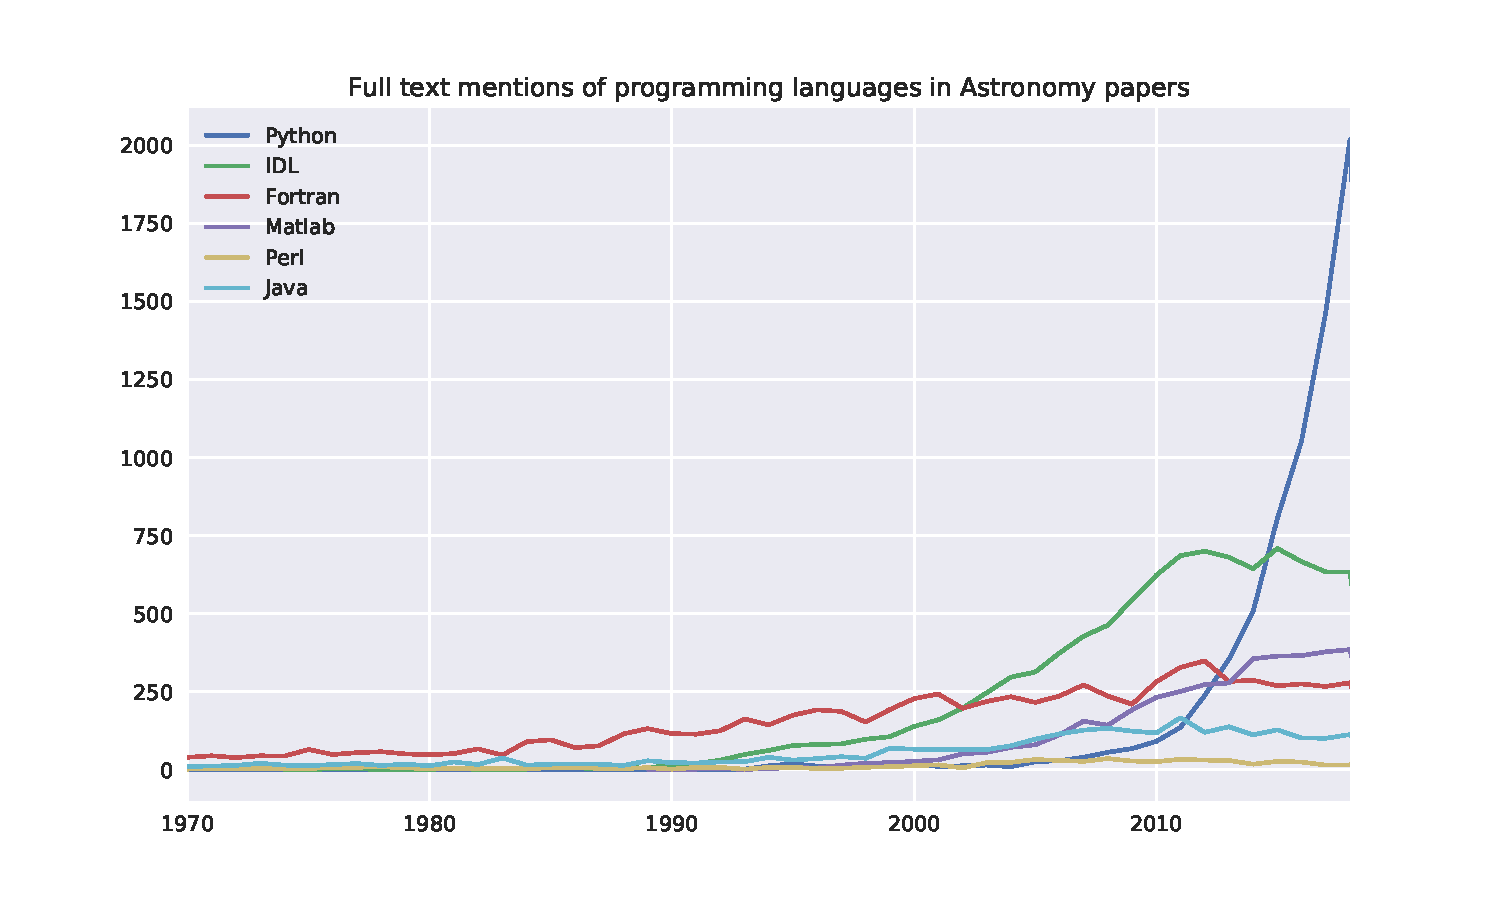
\includegraphics[width=0.8\textwidth]{python-astro-citations}
  \caption{Mentions of programming languages in refereed Astronomy papers, extracted from ADS. Python usage has increased dramatically in the recent years.}\label{fig:python-astro-citations}
\end{figure}

Deliverable: \localdelivref{application-astro}


\end{task}

\begin{task}[
  title=Geosciences application,
  id=geoscience,
  lead=UIO,
  PM=24,
  wphases={0-48},
  partners={QS,SRL}
]

% Scientific description

The amount of geospatial data from a variety of sources, including satellite observations, 4D simulations and in-situ observations, contributed by volunteers
or state agencies keeps increasing. In many disciplines, managing this large volume
has become a challenge, and the old approach of downloading datasets for a local
analysis has become intractable.

The heterogeneity of the tools used in different institutions to deal with
large geographical datasets makes it difficult for researchers to share the outcome
of their work in a reproducible fashion.

In this context, Jupyter is now emerging as a standard exploration tool for
geospatial analysis, climate science, geology and by data providers in these areas.

To mention a few,

\begin{itemize}
\item
   the \emph{PanGeo} platform (Funded by the NSF, NASA, and the Alfred P.
   Sloan Foundation) is built upon Jupyter, JupyterHub, Binder, and Dask.
\item
   the \emph{Joint Research Centre Earth Observation Data and Processing Platform}
   (JEODPP) relies on Jupyter, JupyterHub and ipyleaflet as its main user
   interface.
\item
   the \emph{google earth engine} platform also offers a jupyter-based user
   interface allowing the visual exploration of the data with ipyleaflet.
\end{itemize}

In these three cases, deferred processing is used to restrict computation to
the extent of the area displayed in the map viewer, which allowed these
platforms to scale up to petabytes of data. In all examples, interactive
visualization is a key feature of the platform. Beyond tile-based
2-D visualization, the ability to efficiently process and visualize vector
or 3-D data is also becoming critical.

The BOSSEE team, which comprises the main authors of the technologies upon
which these platforms are built (Jupyter, JupyterHub, Binder, ipyleaflet),
together with the Department of Geosciences of the University of Oslo, are
in a unique position to bring these technologies together in the context of
EOSC.

This demonstrator will focus on tools for two transversal research projects

\begin{itemize}
\item LATICE (Land-Atmosphere Interactions in Cold Environments)
\item EarthFlows (Interface Dynamics in Geophysical Flows)
\end{itemize}

The work items for this demonstrator fall in two main categories:
visualization and geographical data processing tools.

\textbf{Visualization}

\begin{compactitem}
  \item Improvement upon existing mapping tools for specialized
    visualization of in-situ and model-generated data arizing in
    specific use cases (Land, river-runoff, ocean, ice, wave and
    atmosphere models, particle dispersion models, oil spill models,
    etc.).

    This may take the form of additions to the \emph{ipyleaflet} and
    \emph{folium} extentions to JupyterLab, as well as the production of
    curated examples in the documentation of ipyleaflet addressing these
    specific use cases.

  \item Improvements of the tooling for 3-D visualization of
    geographical datasets in the Jupyter notebook, for use cases such as
    displaying volcanic plumes (injection of aerosols in the various
    atmospheric layers), the quasi biennial oscillation (inversion of
    the wind direction in the tropical stratosphere), atmospheric rivers
    (flowing column of condensed water vapour in the atmosphere) and
    also at smaller scales to visualize 3-D discrete particle simulations
    of sheared granular fault zones.
\end{compactitem}

\textbf{Collaboration with Jupyter with specialized tools for earth sciences}

\begin{compactitem}
  \item adding the ability to interactively integrate information or corrections
    observed during field trips, correspdonding to specific geographical locations.

    \TODO{Concurrent editing links to real-time editing from the
    core WP2 - mention link?}

  \item adding the ability to deploy Jupyter-based applications together with
    the correspdonding execution environment, both in the form of a runnable
    notebook with \emph{Binder} or as a read-only yet interactive \emph{Voila}
    dashboard.
\end{compactitem}

\textbf{Teaching geo-sciences with Jupyter}

  All these developments will be used both for scientific research and
  in the classroom for teaching master's students with best practices
  in open science.

  The Geosciences use case will make it possible to demonstrate the
  effectiveness of the BOSSEE co-design approach. The main challenges
  will be on the one hand to learn to take advantage of feedback given
  by users (either novices or experts) and on the other hand for
  BOSSEE developers to adapt their communication and language as well
  as their offer to the Geoscience. This will lead the way for
  on-boarding new communities.

  \TODO{The transversal research plays into the desired ``services that
    encourate collaborative interdisciplinary work'' that are desired
    by this call; this is good. Can you imagine that some of these
    facilities can be used via the EOSC? That would be a good
    addition. For example, one could use the BinderHub installation
    that we expect on the EOSC. }


\end{task}

\begin{task}[
  title=Application Interactive Mathematics with Jupyter Widgets,
  id=math,
  lead=UPSUD,
  PM=16,
  wphases={0-36},
  partners={UPSUD,QS}
  ]

  Computations have played a long time and ever increasing role for
  research and teaching in (pure) mathematics, to explore, search and
  check for conjectures, or better understand algorithmic ideas. This
  led to the development of a whole ecosystem of mathematical
  software, many of which are open source. Given the huge variety of
  mathematical objects and workflows, the Read-Eval-Print-Loop (REPL)
  paradigm -- on which Jupyter is based -- is particularly suitable:
  the user interacts with the system by typing commands that use its
  library of mathematical features, often combined with personal code.
  In fact, the REPL and notebook paradigms of Jupyter as well as some
  of its interactive features were largely inspired by that of
  computer algebra systems such as Maple, Mathematica, or SageMath.

  One major action of the OpenDreamKit project was to foster the
  convergence between the Jupyter and math software ecosystems:
  nowadays Jupyter can be used as a uniform user interface for most
  major systems: e.g. GAP, OSCAR, Pari/GP, SageMath, Singular, and
  even for C++ libraries. This interface is being widely adopted: for
  example, Jupyter has become the standard user interface for
  SageMath, enabling to phase out its former bespoke notebook.

  By itself, this enables all the advantages of the upcoming
  EOSC-based generic Jupyter services to the mathematical community.

  The next step to maximize attractivity and impact in the
  mathematical community, and this is the aim of this task, is to go
  beyond the REPL paradigm, and \textbf{leverage the real time
    interactivity and flexibility brought by Jupyter widgets for
    Mathematical purposes}. Think making it easy for a teacher or
  researcher to build and disseminate a mini applications or dashboard
  enabling to explore graphically a whole range of mathematical inputs
  and visualizing in real time associated outputs.

  The unique challenge comes from the huge variety of mathematical
  objects that the user may want to visualize and interact with, and
  the variety of graphical representations. Co-design is central here,
  as building a bespoke interactive visualization entails a
  combination of technology skills (e.g. javascript development) and
  business knowledge (designing the interaction and visualization).
  The role of Research Software Engineers is to leverage the
  technology by encapsulating the technical difficulties into flexible
  and easy to use tool boxes from which mathematicians can build
  mini-applications tailored to their needs.

  Within OpenDreamKit, we conducted experiments to explore this
  venue~\cite{ODK_D4.16}. One specific focus was to enable not only
  \emph{interactive visualization}, but also \emph{interactive
    editing}: being able to graphically modify the mathematical object
  being visualized; this enable the interactive exploration of how the
  modifications affect its properties, or to use the editor as input
  widget for a larger applications or dashboards. The outcome of this
  task are the development of two prototypes in SageMath
  (\software{sage-combinat-widget}, a library of widgets for
  combinatorics, and \software{sage-explorer} a generic dashboard for
  interactive browsing and introspection of mathematical objects), and
  contributions to \software{Francy}, an Interactive Discrete Math
  Framework for \software{GAP} and \software{SageMath}.

  The aim of this task is to build on this experience to further
  develop and promote the use of Jupyter widgets for interactive
  Mathematics. This will include the following actions:
  \begin{compactitem}
  \item Engage with the community through tutorials, workshops, online
    discussions, for codesign and for dissemination of the outcomes.
  \item Tackle hurdles to real-time interactivity, typically by
    modernizing the existing 2D and 3D visualization tools in
    SageMath. % E.g.: We don't use Matplotlib's integration in Jupyter
  \item Bring \software{sage-combinat-widgets} and
    \software{sage-explorer} from usable prototypes to standard tools,
    and further contribute to the development of the \software{Francy}
    framework.
  \item Develop other generic mathematical widgets according to the
    users popular requests.
  \item Demonstrate the value all of the above through applications in
    research and teaching.
  \end{compactitem}
  The work carried over will be reported on in~\localdelivref{math}.
\end{task}

\begin{task}[
  title=Nuclear Medicine application,
  id=opendose-analysis,
  lead=INSERM,
  PM=24,
  wphases={0-24},
  partners={}
]
  % Scientific description
  Nuclear Medicine is a field of medicine where radioactive material
  (radiopharmaceutical) is used for diagnostic and therapy. Even though the
  majority of Nuclear Medicine procedures (90\% according to successive EANM
  surveys) are diagnostic examinations, therapeutic applications tend to
  develop and drag more and more attention, for example for the treatment of
  neuroendocrine tumours \cite{Bodei2009}.

  The formalism used to objectively characterise the irradiation process is
  similar for both application types: it was introduced in the late 60s by the
  MIRD (Medical Internal Radiation Dose) committee of the American Society of
  Nuclear Medicine (SNM). This formalism \cite{loevinger1991mird} requires two
  independent quantities; the radioisotope cumulated activity ($Bq.s$) in the
  source (tissue/organ) and the mean absorbed dose to a given target
  (tissue/organ) per radioisotope disintegration (S-value,
  $Gy.Bq^{-1}.s^{-1}$). The S-value calculation requires a clear definition of
  the geometry of the patient (or the model) and radioisotope decay
  characteristics, it can be expressed as a linear combination of
  yields/energies ($J$) and Specific Absorbed Fractions (SAF, $g^{-1}$).

  The calculation of SAFs involves radiation transport modelling and energy
  deposition scoring in anthropomorphic models, usually based on Monte Carlo
  simulation. Historically, SAFs were computed from mathematical models -
  simplistic approximations to human geometry. The advent of voxel-based
  computational models requires a new appraisal of dosimetric data. For
  example, the models recently proposed by the International Commission on
  Radiation Protection (ICRP) include 140 possible radiation sources, leading
  to around 20000 source/target combinations \cite{ICRP2009ICRPPhantoms}. The
  production of SAFs for these models for all possible source regions,
  radiation types and energiesimpul represent an important computation time
  (millions of CPU hours).

  The OpenDose project \cite{Chauvin2017} is a collaborative effort to generate
  reference dosimetric data using various Monte Carlo codes across different
  teams. The collaboration includes at the moment 14 research teams over 18
  institutes.  The idea is to trigger the collaborative development of a
  reference database, freely available, proposing dosimetric data applicable in
  a context of nuclear medicine dosimetry (for therapy and diagnostic
  applications). A major aspect of the project is the development of tools
  ensuring traceability and robustness of generated results.

  % Technical description
  OpenDose data is produced using the five most represented Monte Carlo
  simulation software in medical applications: Geant4/GATE, MCNP, EGS, PENELOPE
  and Fluka. Each simulation consists of calculating radiation transport in
  anthropomorphic models for specific parameters (source organ, particle type,
  energy, model and number of primaries to simulate). Every simulation produces
  binary (3D matrices) and ASCII files for a total of $\sim$150MB / simulation.
  The 3D matrices contain energy deposited per voxels, and ASCII files contain
  pre-processed data corresponding to energy deposited per regions such as
  organs and tissues. These raw outputs are later processed into dosimetric
  data such as Specific Absorbed Fractions (SAFs) and S-values.

  Producing data for one model (ex. adult female) requires $\sim$30,000
  simulations, with the workload shared between the different teams and
  software.

  The data produced by all the teams is currently centralised at the Cancer
  Research Center of Toulouse (CRCT), processed and fed into a local SQL
  database at CRCT.

  This collaborative effort raises some challenges:
  \begin{compactitem}
  \item Data production: a total of 750,000 hours of CPU time is needed per
    model.
  \item Volume of data: one model represents TB of raw data that can be
    heterogeneous from the different teams.
  \item Data analysis: raw data has to be processed into dosimetric data in a
    robust and reproducible way.
  \item Database: has to be efficient and handle all the data (raw and
    processed).
  \item Visualization: display and compare results from all teams.
  \end{compactitem}

  The objective of this task is to build on the Jupyter ecosystem to create a
  unified data analysis framework for the OpenDose project. By building a set
  of tools to access and process data, this will ensure the production of
  traceable and reproducible dosimetric data for the OpenDose project members.

  Another major aspect of the OpenDose collaboration is to provide an open
  access to the generated dosimetric data. For that purpose a website is under
  development to allow data download and simple dosimetry calculations. For
  users who need more advanced calculations, a dedicated Jupyter workspace will
  provide a set of tools to easily access, process and display the OpenDose
  data.

  The task includes the following activities:
  \begin{compactitem}
  \item Developing tools to work seamlessly on the SQL database holding the
    dosimetric data.
  \item Developing data analysis tools using the Python data science ecosystem
    where possible.
  \item Developing visualization tools, exploring Widgets inside the Notebook
    for interactivity.
  \item Comparing results between teams. \TODO{Which teams and what
      results? Scientific work itself is not in the remit here?}
  \item Disseminating results.
  \item Providing support to users.
  \end{compactitem}
  These developments will be integrated in the demonstrator
  (\localdelivref{opendose-analysis})

  \TODO{Can the demonstrator run on the EOSC hub, or be ported in
    principle? If not, what is the link? Is this a service that could
    be made available via the EOSC hub if it turns out to be useful?}


  \TODO{Are there other communities with similar needs?}

  \TODO{How does this task relate to EOSC-life?}

\end{task}

\begin{task}[
  title=Application: Visualisation and control of fluid dynamics in Jupyter notebook,
  id=application-gpu,
  lead=SIL,
  PM=13,
  wphases={4-36},
  % don't include lead here
  partners={EGI}
]

\textbf{Context: Fluid dynamics with Lattice Boltzmann method on GPU}

In recent years, the lattice Boltzmann method (LBM) emerged as an
interesting alternative to more established methods for fluid flow
simulations. Sailfish-cfd \cite{januszewski2014sailfish} is an open
source implementation of LBM on General Purpose Graphical Processing
Unit (GPGPU) devices. It is written in Python with real-time
generation of CUDA-C code.  In order to harvest capabilities of GPGPU
one needs to access the specialized hardware, which usually is
avaiable to researchers as remote HPC resources.  The typical fluid
dynamics research workflow consists of three stages: preparing
boundary conditions, running a simulation, and data analysis. The
first and last stage require capable and responsive user interface for
maniputation and inspection of 3d data.  The Jupyter 3d visualization
widgets developed in \taskref{ecosystem}{jupyter-widgets} can fulfill
such needs.

\textbf{This task}

In this task we will improve and adapt existing open software to
easily work in Jupyter notebook and fully use its interactive
features. Based on previous experience with K3D-jupyter\cite{K3D}
widget we know that web browser based software can display moderate
dataset during the simulation As the dataset is becoming larger the
visualization in the browser turns out to be nontrivial due to
limitations of the browser itself and large data transfers. There is
an open question on how much of data processing should be performed on
server-side and what can be done on the widget (browser side). Our
experience suggests that there is no clear answer and it depends on
the size of the data and its nature. For example, volume rendering
technique if very effective on the browser side but infers large data
transfers. One can perform it the server-side, in a distributed way if
the simulation uses many nodes, but the interactivity is limited by
network latency. In this task we will attempt to provide practical
solution to this issue.  Furthermore, we will contruct tools for
editing and inspecting boundary conditions. Having such tools as
Jupyter widgets will allow to complete the workflow without leaving
Jupyter notebook.

The task includes the following activities

\begin{compactitem}
\item Development of Jupyter notebooks using LBM based fluid
  simulation based on the high-performance Sailfish-cfd solver.
\item Implementing advanced widgets for data visualization of large
  fluid dynamics simulations.
\item Implementing widgets for inspection and editing boundary
  conditions in LBM.
\end{compactitem}

This part will closely interact in with the task
\taskref{ecosystem}{jupyter-widgets}: it will both provide guidelines
for the development to \taskref{ecosystem}{jupyter-widgets} and serve
as test case for implemented features in
\taskref{ecosystem}{jupyter-widgets}.

The deliverable of this part will be a demonstrator
(\localdelivref{lbm-jupyter}) available via the EOSC hub.

\end{task}

\end{tasklist}



\begin{wpdelivs}
%\TODO{update due date and startup!}
\begin{wpdeliv}[due=42,miles=community,id=application-astro,dissem=PU,nature=DEM,lead=CDS]
    {Demonstrator of astronomical data services based on on reference astronomy data from CDS in Jupyter notebooks is made available for use by the astronomy research community.}
\end{wpdeliv}
\begin{wpdeliv}[due=45,miles=final,id=xfel-workflows,dissem=PU,nature=DEM,lead=XFEL]
  {Demonstrator reproducible photon science}
\end{wpdeliv}

% \TODO{update milestone!}
\begin{wpdeliv}[due=36,miles=final,id=math,dissem=PU,nature=R,lead=UPSUD]
  {Report on Interactive Mathematics with Jupyter Widgets}
\end{wpdeliv}
\begin{wpdeliv}[due=48,miles=final,id=applications-report,dissem=PU,nature=R,lead=XFEL]
  {Evaluation of demonstrators and case studies. Report on
    feasibility, user feedback, potential shortcomings and
    improvement, to guide EOSC service design.}
\end{wpdeliv}
\begin{wpdeliv}[due=24,miles=final,id=lbm-jupyter,dissem=PU,nature=DEM,lead=SIL]
  {Demonstrator of simulations  SDE based research in Jupyter notebook. It will include example reproducing recent research as well as tutorial for researcher and developers.}
\end{wpdeliv}
\begin{wpdeliv}[due=36,miles=final,id=sde-jupyter,dissem=PU,nature=DEM,lead=SIL]
  { Demonstrator of LBM simulation in in Jupyter notebook using GPU solver sailfish-cfd. It will include setting boudary conditions, monitoring the simulation and visualisation of the data. It will be based on K3D-Jupyter widget for 3d interactive input and output.}
\end{wpdeliv}


\begin{wpdeliv}[due=36,miles=final,id=opendose-analysis,dissem=PU,nature=DEM,lead=INSERM]
  {Jupyter services for nuclear medicine dosimetry with the OpenDose project}
\end{wpdeliv}

\begin{wpdeliv}[due=48,miles=final,id=teaching,dissem=PU,nature=R,lead=EP]
  {How Jupyter ecosystem can enrich the teaching experience: a case study at \'Ecole polytechnique and Université Paris-Sud.}
\end{wpdeliv}

\end{wpdelivs}
\end{workpackage}
%%% Local Variables:
%%% mode: latex
%%% TeX-master: "../proposal"
%%% End:

%  LocalWords:  workpackage wphases wpobjectives wpdescription pageref wpdelivs wpdeliv
%  LocalWords:  dissem mailinglists swrepository final-mgt-rep compactitem swsites ipr
%  LocalWords:  TOWRITE tasklist delivref
\newpage
\TOWRITE{ALL}{Proofread WP 1 Management pass 1}
\begin{draft}
\TOWRITE{PS (Work Package Lead)}{For WP leaders, please check the following (remove items
once completed)}
\begin{verbatim}
- [ ] have all the tasks in this Work Package a lead institution?
- [ ] have all deliverables in the WP a lead institution?
- [ ] do all tasks list all sites involved in them?
- [ ] does the table of sites and their PM efforts match lists of sites for each task?
      (each site from the table is listed in all relevant tasks, and no site is listed
      only in the table or only at some task)
\end{verbatim}
\end{draft}

\begin{workpackage}[id=eosc,wphases=0-48,swsites,
  title=Services and EOSC Integration,
  short=EOSC,
  lead=SRL,
  EGIRM=21,
  EPRM=6,
  % INSERMRM=4,
  % QSRM=6,
  % SILRM=4,
  SRLRM=18,
  % UIORM=12,
  UPSUDRM=4,
  WTTRM=15,
  XFELRM=6,
]
\begin{wpobjectives}
 \begin{compactitem}
   \item operate services for open science
   \item migrate services to EOSC
 \end{compactitem}
\end{wpobjectives}

\begin{wpdescription}

This work package is about the actual operation of services developed in the other work packages.

\TOWRITE{MORE}

\end{wpdescription}

\begin{tasklist}
% add tasks from task directory here
% % template for a task
% each task should be added to exactly one workpackage
% in the workpackage task list
\begin{task}[title=Task title,
  id=task-id,
  lead=XXX,
  PM=1,
  wphases={0-48},
  partners={XXX,SRL}
]
  The task includes the following activities
  \begin{compactitem}
  \item ...
    (\delivref{workpackage}{deliv-id})
  \end{compactitem}
\end{task}

% template for a task
% each task should be added to exactly one workpackage
% in the workpackage task list
\begin{task}[
  title=Prototype European Binder instance and global federation,
  id=eu-binder,
  lead=SRL,
  PM=21,  % SRL: 12PM, EGI: 3PM, WTT: 6PM, UPSud: 0PM
  wphases={0-48},
  partners={EGI,WTT,UPSUD}
]

  The purpose of this task is to create a community of practice of BinderHub
  operators and operate a European Binder instance.

  Re-executing the code associated with all European Open Access publications
  requires a very large amount of very diverse compute resources. It is
  unrealistic that one BinderHub instance could provide all of these. This is
  why in this task we will work on building a community of practice around
  operating public Binder instances at a research institution.

  Constraints from data protection and privacy mean not all code supporting a
  publication can be made public and/or that data can not be moved outside of
  the EU. This task will work on operating a EU based Binder instance accessible
  to the public. This will mirror the current mybinder.org but be hosted in
  the EU. This European Binder instance will serve as the first partner in the
  global federation of Binder instances.


  \begin{compactitem}
  \item Build a community of practice of BinderHub operators. Create a forum
  for Binder operators to exchange experience and tools.

  \item Operate a Binder instance hosted in Europe.

  \item Develop a federation of Binder instances and produce a report on best
    practices for coordinating several federated BinderHub instances across
    institutes.
    (\localdelivref{eu-binder-instance})
  \end{compactitem}
\end{task}

% template for a task
% each task should be added to exactly one workpackage
% in the workpackage task list
\begin{task}[
  title=Collaboration with EOSC,
  id=eosc,
  lead=EGI,
  PM=33,
  wphases={12-48},
  partners={SRL,XFEL,WTT}
]
  The task includes the following activities

  \begin{compactitem}
  \item Cooperation with existing EOSC projects
  \item make services accessible from EOSC
    (\localdelivref{deliv-id})
  \end{compactitem}
\end{task}

\begin{task}[
  title=Easy deployment of JupyterHub and BinderHub on a variety of
  infrastructure,
  id=jh-bh-deployment,
  lead=EP,
  PM=10, % EP: 11PM
  wphases={0-18}, % ???
  partners={UPSUD,SRL,WTT}]

  The JupyterHub or BinderHub installation tutorials mostly focuses on
  deployment on corporate cloud services (mainly GoogleCloud). For many academic
  institutions and SMEs, a deployment on their own infrastructure is preferable
  for a combination of reasons (better control on private data, easier
  integration with the local information system, the difficulty of funding the
  costs of external services, ...).

  There are many pre-existing academic clouds managed by people with a high
  level of expertise and a thorough knowledge of their infrastructure and
  associated tools. These are often more cost-effective for research and
  education. This is also true for SMEs. The purpose of this task is to make the
  deployment of JupyterHub or BinderHub easier upon these academic cloud
  computing and to provide scalable and high-quality infrastructure for
  education and research. Most of them are based on two open-source softwares
  which can manage this kind of infrastructure: OpenStack and OpenShift. We will
  then focus on these two tools.
  
  While platforms such as GoogleCloud already offer effective tools to deploy a
  Kubernetes cluster, this is not the case when we deploy our own
  infrastructure. The tools available for the two solutions mentioned above are
  numerous and it is often difficult to choose which ones are the most suitable
  and best maintained. We will therefore first take an interest in making a
  state of the art and explaining our choices. We already began this study at
  Ecole polytechnique (see the post in
  medium\footnote{\url{https://blog.jupyter.org/how-to-deploy-jupyterhub-with-kubernetes-on-openstack-f8f6120d4b1}})
  and we want to deepen it. At each step, we will use infrastructures available
  locally (OpenShift at Ecole polytechnique and OpenStack at University of
  Paris-Sud), available in France (OpenShift at Mathrice which is a "Groupements
  de Service" at CNRS of the research laboratories IT in French mathematics),
  available in Europe (EGI). We will document all the process to allow the
  community to easily deploy a JupyterHub or BinderHub on their own
  infrastructure based on OpenStack and/or OpenShift.

  Once the infrastructure is in place, even if JupyterHub or BinderHub provide
  efficient teaching or research environments, one issue remains: the lack of
  choice in terms of storage devices and data persistence. Thus, we will provide
  a unified environment and  focus on the possibility to mount various  storage
  devices on the containers deployed on the Kubernetes cluster and provide
  persistence storage for Binder. This will be a key issue for the task
  \taskref{core}{jh-bh-conv}.
  
  The task includes the following activities:
  \begin{compactitem}
  \item Prototypes / POC deployment on OpenStack and/or OpenShift
  \item Partial / Full automation of the deployment
  \item Documentation ($\rightarrow$
  \localdelivref{openstack-openshift-documentation})
  \end{compactitem}
\end{task}

\end{tasklist}




\begin{wpdelivs}
\begin{wpdeliv}[due=1,miles=startup,id=infrastructure,dissem=PU,nature=DEC,lead=SRL]
  {Some Deliverable}
\end{wpdeliv}

\end{wpdelivs}
\end{workpackage}
%%% Local Variables:
%%% mode: latex
%%% TeX-master: "../proposal"
%%% End:

%  LocalWords:  workpackage wphases wpobjectives wpdescription pageref wpdelivs wpdeliv
%  LocalWords:  dissem mailinglists swrepository final-mgt-rep compactitem swsites ipr
%  LocalWords:  TOWRITE tasklist delivref
\newpage
\TOWRITE{ALL}{Proofread WP 1 Management pass 1}
\begin{draft}
\TOWRITE{PS (Work Package Lead)}{For WP leaders, please check the following (remove items
once completed)}
\begin{verbatim}
- [ ] have all the tasks in this Work Package a lead institution?
- [ ] have all deliverables in the WP a lead institution?
- [ ] do all tasks list all sites involved in them?
- [ ] does the table of sites and their PM efforts match lists of sites for each task?
      (each site from the table is listed in all relevant tasks, and no site is listed
      only in the table or only at some task)
\end{verbatim}
\end{draft}

\begin{workpackage}[id=education,wphases=0-48,swsites,
  title=Education and Dissemination,
  short=Education,
  lead=INSERM,
  CDSRM=3,
  % EGIRM=4,
  % EPRM=TBC,
  INSERMRM=12,
  QSRM=4,
  SILRM=5,
  SRLRM=13,
  UIORM=12,
  UPSUDRM=3,
  WTTRM=3,
  XFELRM=8,
  EPRM=3,
]
\begin{wpobjectives}
  The objective of this work package is to develop the community at the
  European scale, foster cross team collaboration, spread the
  expertise, and engage the greater community to participate in the
  definition and refinement of the requirements, and the implementation and use of the
  produced solutions. This includes:
 \begin{compactitem}
   \item Ensure awareness of the results in the user community;
   \item Train researchers in best practices for open and reproducible science
   \item Educate the community on the value of open science
   \item Produce training and education material to disseminate the ability to do reproducible computational science using the tools we develop.
   \item Define individual exploitation plans;
 \end{compactitem}
\end{wpobjectives}

% Potential sources of inspiration: ODK's WP2 work package about dissemination:
% PDF: p.36 of https://github.com/OpenDreamKit/OpenDreamKit/raw/master/Proposal/proposal-www.pdf
% Sources: https://github.com/OpenDreamKit/OpenDreamKit/blob/master/Proposal/WorkPackages/DisseminationCommunityBuilding.tex

\begin{wpdescription}

Open science is entirely dependent on researchers adopting open practices.
In \TheProject, we are developing tools to facilitate these practices,
but they only work if researchers actually adopt them.
Going further, it is also clear that open science is not just of value
to researchers: one of the largest benefits of open science is that it makes
science accessible to the broader public who may not be members of the
research community.

To this end, in addition to training researchers, we will also train the public in how to
make use of the open science research and services facilitated by \TheProject.
This will be done through regular open dissemination and training workshops, as well as
by producing and maintaining material for online courses and documentation.

\TheProject will develop, through WP4, a number of applications and demonstrators that
will be disseminated in different ways.
We will also participate in the concertation activities,
consultations and other meetings and events of the European
E-Infrastructure projects.

All the code, documents, test and build infrastructure produced as
part of the project will be made available as open source.
Open access to all publications resulting from the project will be ensured.


\end{wpdescription}

\begin{tasklist}
% add tasks from task directory here
% template for a task
% each task should be added to exactly one workpackage
% in the workpackage task list
\begin{task}[
  title=Dissemination and communication activities,
  id=website,
  lead=SRL,
  PM=12,
  wphases={0-48},
  partners={XFEL,QS,WTT,SIL,INSERM,UPSUD}
]

% flat copy/paste from similar task in ODK proposal
This task comprises all forms of direct dissemination and public
communication activities such as press releases, creation of the
project web-site including visitor analysis and monitoring tools,
scientific and technical publications, outreach activities
(seminars, keynote talks, media interviews, press releases),
promotion through social media (e.g. Twitter, Facebook, LinkedIn),
creation of advertisement materials such as flyers, posters, and
electronic feeds as well as their distribution. We will use standard
community building technology such as mailing lists, Wikis and
Forums, to ensure dissemination and engagement of the community to
support this. We will also generate press releases at appropriate
moments.

\end{task}

% template for a task
% each task should be added to exactly one workpackage
% in the workpackage task list
\begin{task}[
  title=Training Workshops and community building,
  id=workshops,
  lead=UIO,
  PM=35, % UPSUD: 1PM
  wphases={0-48},
  partners={SRL,XFEL,QS,CDS,WTT,SIL,UPSUD,EP,INSERM}
]
This task will be in charge of:

 
  \begin{compactitem}

   \item Defining and implementing a strategy to enable a shared vision of the Jupyter ecosystem across all the actors from developers, users to every stakeholder: the current misalignment hinders the full exploitation of Open Software practices where co-design is a de facto approach.

For instance, the official Jupyter documentation (https://jupyter.org/documentation) solely reflects the view of developers where the Jupyter ecosystem is defined as a set of software packages (jupyter-core, jupyter-client, kernels, widgets (ipywidgets, ipyleaflet, etc.). The user vision is relegated to examplars (blogs, newsletters, etc.) which inevitably tend to be restrictive but often become de facto standards. This can lead to misconceptions and makes it more difficult for on-boarding novices and new communities.


\item Triggering a cultural change to help under-represented groups to actively participate to the development of open source project to ensure the sustainability of the \TheProject services deployed on EOSC-HUB. 
 

\item Foster Open innovation by collaborating with others from different background and activities (school, universities, industries, journalists, artists, etc.)

  \end{compactitem}
 

To achieve these goals, the following actions/activities will take place:


  \begin{compactitem}
   \item co-design hackathons: the co-design efforts between domain scientists, \TheProject developers and service providers will be carried out at any point in time of the project and will be registered in a co-design register to help for future engagement with new communities of users. To be fully effective,  co-design hackathons will be organized to set the stage, define rules for co-design interactions and more importantly align all actors into a common user-centred vision of \TheProject services and associated development towards a successful EOSC deployment. 


   \item Workshops on Findable, Accessible, Interoperable and Reusable (FAIR) software and data to facilitate the adoption of Open Science best practices (transparent, sharable and collaborative Science): this would not be restricted to the Jupyter ecosystem and will teach users how to make data, lab notes and other research processes freely available, under terms that enable reuse (licensing), redistribution and reproducibility of methods and/or results.

   \item Trainings on how to use \TheProject software and services to fully exploit \TheProject developments for EOSC: develop training materials and organize training events for researchers and the public to enable Open Science and maximise the usefulness of \TheProject developments.

   \item \TheProject Admin trainings: training event for learning on how to deploy \TheProject services such as BinderHub.


   \item Open call for open innovation mini-projects: mentored by \TheProject staff and targeting SMEs, municipalities, journalists, artists, etc.

  \end{compactitem}
 
    (\localdelivref{workshops})
\end{task}

% template for a task
% each task should be added to exactly one workpackage
% in the workpackage task list
\begin{task}[
  title=Online resources for open science,
  id=online-resources,
  lead=INSERM,
  PM=14,
  wphases={0-48},
  partners={SRL,XFEL,QS,CDS,WTT,SIL,UPSUD,EP}
]
  The task includes the following activities
  \begin{compactitem}
  \item The interactive book on applied Stochastic processes in Physics. Unlike classical books in this subject, it will be supplemented by numerical examples of solving real case problems. We will emphasize the
role of high performance computing in solving problems modeled by stochastic differential equations (SDE). Materials will contain examples of using GPU computing in solving SDE. The deliverable of this part will be available via the EOSC hub, and will use HPC hardware available. (\localdelivref{sde-book})
  \end{compactitem}
\end{task}

\begin{task}[
  title=Local Help Desk,
  id=helpdesk,
  lead=UPSUD,
  PM=3PM, % UPSUD=2PM, Simulate=1PM
          % please update according to your site involvement,
  wphases={0-48}, % At Paris-Sud, and unless complemented by other
                  % funding, this will stop after 18 months
  partners={SRL,XFEL,QS,CDS,WTT,SIL,UPSUD,INSERM,EP}
  ]

  Dissemination events and tutorials are very effective tools for
  engaging scientists and giving them the desire to acquire new
  technologies and best practices. The next barrier to adoption comes
  when, back home, the scientists start using them on their daily
  problem. Having access to a local expert -- even for a small amount
  of time -- makes a huge difference, saving on the wasted time and
  frustration on the inevitable rough corners, and getting first hand
  advice and guidance in the rich landscape of available tools that
  could otherwise soon feel overwhelming.

  At several of our sites, our Research Software Engineers will
  dedicate some fraction of their time to deliver such help to the
  local community, experimenting with various formats: help desk hours
  where scientists can drop by to get help; regular meet-ups where
  scientists can reconvene to work on their problems or on-demand
  tutorials with expert supervision and mutual help; in-lab visits to
  the scientists for more in-depth discussions; etc.

  An explicit aim of this task is to foster the creation of
  sustainable Research Software Engineer groups within institutions to
  support their scientists.

  This will be the occasion for our Research Software Engineers to
  witness first hand how users adopt or struggle with the projects
  technologies and services, and escalate the hurdles and barriers to
  adoptions as well as success stories. The sites will keep in close
  contact to exchange on the effectiveness of the various formats, and
  the outcome will be reported on in deliverables
  \localdelivref{report1}, \localdelivref{report2}, \localdelivref{report3}.
\end{task}

\end{tasklist}


\TODO{Choose milestone for each report}
\begin{wpdelivs}
\begin{wpdeliv}[due=18,id=report1,dissem=PU,miles=xxx,nature=R,lead=INSERM]
  {Community building: Impact of development workshops, dissemination and training activities, reporting period 2}
\end{wpdeliv}
\begin{wpdeliv}[due=36,id=report2,dissem=PU,miles=xxx,nature=R,lead=INSERM]
  {Community building: Impact of development workshops, dissemination and training activities, reporting period 2}
\end{wpdeliv}
\begin{wpdeliv}[due=48,id=report3,dissem=PU,miles=xxx,nature=R,lead=INSERM]
  {Community building: Impact of development workshops, dissemination and training activities, reporting period 2}
\end{wpdeliv}
\end{wpdelivs}

\end{workpackage}
%%% Local Variables:
%%% mode: latex
%%% TeX-master: "../proposal"
%%% End:

%  LocalWords:  workpackage wphases wpobjectives wpdescription pageref wpdelivs wpdeliv
%  LocalWords:  dissem mailinglists swrepository final-mgt-rep compactitem swsites ipr
%  LocalWords:  TOWRITE tasklist delivref
\newpage
\end{workplan}

\ifgrantagreement
\endgroup
\setcounter{page}{\value{savepage}}
\fi

%%% Local Variables:
%%% mode: latex
%%% TeX-master: "../proposal"
%%% End:

%  LocalWords:  newpage workpackages workplan



%%% Local Variables:
%%% mode: latex
%%% TeX-master: "proposal"
%%% End:
